\documentclass{sig-alternate}

\usepackage{amsmath,mathtools,nccmath}
\usepackage{paralist,url}
\usepackage{bigints}
\usepackage{tikz}
\usetikzlibrary{matrix,arrows,shapes,calc}

\newtheorem{example}{Example}
\newtheorem{definition}{Definition}
\newtheorem{theorem}{Theorem}

\newcommand{\ite}[3]{\mathbf{if}\ #1\ \mathbf{then}\ #2\ \mathbf{else}\ #3\ \mathbf{fi}}
\newcommand{\pvec}[1]{\vec{#1}\mkern2mu\vphantom{#1}} %for primed vector (by egreg)
\newcommand{\abs}{\ensuremath{\mathrm{abs}}}
\newcommand{\sign}{\ensuremath{\mathrm{sign}}}


\begin{document}

\title{Evaluating PALS with SMT on a Distributed Nonlinear Airplane Turning Controller
%\titlenote{For use with ACM\_PROC\_ARTICLE-SP.CLS. Supported by ACM.}
}

\numberofauthors{3}
\author{
Kyungmin Bae, Sicun Gao, Edmund M. Clarke\\
\affaddr{Department of Computer Science}\\
\affaddr{Carnegie Mellon University}
}

\maketitle
\begin{abstract}
We evaluate the performance of SMT-based analysis on a distributed
nonlinear aircraft controller. Such a model has been studied using
techniques from ..., but there are limitations such as... We show how
to generate SMT formulas to solve problems in the PALS framework and
evaluate the scalability of state-of-the-art SMT solving techniques on
these problems. We also give directions for improvement on SMT for
handling more general properties like ....
\textbf{TO BE WRITTEN}
\end{abstract}

%%%%
%%%%
\section{Introduction}

\textbf{TO BE WRITTEN}

\newpage


%%%
\subsection{Related Work}

The Multirate PALS model of the distributed airplane
turning controller was introduced \cite{ftscs-journal}.
Both liveness and safety properties of the airplane controller was analyzed,
based on explicit-state model checking in Real-Time Maude \cite{journ-rtm}.
These analyses only considered  specified pilot behaviors and system parameters,
and used numerical simulations to deal with nonlinear differential equations.
%
On the contrary, 
this paper applies $\delta$-complete SMT solving 
to analyze the airplane controller
for arbitrary pilot behaviors and bounds of system parameters,
and to deal with nonlinear differential equations up to 
up to any precision $\delta > 0$.
The synchronous model $\mathcal{E}$ 
is also modified from \cite{ftscs-journal} to precisely model
the physical correlations between distributed controllers,
rather than using approximations as did in \cite{ftscs-journal}.
For the Multirate PALS methodology,
we refer to \cite{ftscs-journal,mr-pals-journal,pals-tcs} for details.

Distributed hybrid systems for avionics have been much studied
in the context of collision avoidance maneuvers for a set of airplanes
(e.g., see \cite{loos-hscc13} and the references therein).
However, we are not aware of hybrid system models for a turning 
controller of an airplane to move the ailerons and rudder.
Such a coordinated turn is essential for fly-by-wire control systems,
and is an elemental topic in aeronautics \cite{anderson2005introduction}.



\textbf{Sean, could you add some related work on \texttt{dReal}, or SMT for hybrid systems,
if necessary?}




\newpage



%%%%
%%%%
\section{Preliminaries}

%%%
\subsection{Multirate PALS} 

The Multirate PALS (``physically asynchronous,  logically synchronous'') 
methodology \cite{pals-rtss09,mr-pals-journal,pals-tcs}
aims at reducing the system complexity 
of \emph{virtually synchronous}  cyber physical systems (CPS),
such as airplanes and cars,
implemented as a network of multirate distributed components but essentially designed in a synchronous way.
%
The design and verification of a virtually synchronous CPS
is challenging  due to
clock skews,
execution times, 
network delays, and asynchronous communication,
plus the state space explosion caused by the system's concurrency. 
%
Multirate PALS can reduce
the design and verification of a virtually synchronous CPS to
that of its much simpler synchronous counterpart,
provided that the underlying infrastructure provides bounds $\Gamma$
on the skews of the local clocks, 
execution times,  and network delays. 
%
Given a synchronous design $\mathcal{E}$ and a global period $T$,
Multirate PALS generates
the corresponding distributed asynchronous 
design $\mathcal{A}(\mathcal{E}, T, \Gamma)$
in which both $\mathcal{E}$ and $\mathcal{A}(\mathcal{E}, T, \Gamma)$
satisfy the same temporal logic properties \cite{mr-pals-journal,pals-tcs}.
%
%By simply designing and verifying a synchronous model $\mathcal{E}$,
%Multirate PALS %can automatically 
%gives the \emph{correct-by-construction}  
%implementation  $\mathcal{A}(\mathcal{E}, T, \Gamma)$.



The multirate synchronous model $\mathcal{E}$ 
is formally specified as
a synchronous composition of a set of  nondeterministic state machines \cite{pals-tcs}.
%
A \emph{typed machine} with $n$ input ports and $m$ output ports
is a tuple $M = (D_i,S,D_o,\delta_M)$,
where
$D_i = D_{i_1} \times \cdots \times D_{i_n}$ is an input set 
(a value to the $k$-th \emph{input port}  is an element of $D_{i_k}$ for $1 \leq k \leq n$), %
$S$ is a finite set of states,
$D_o =D_{o_1} \times \cdots \times D_{o_m}$ is an output set
(a value from the $j$-th \emph{output port} is an element of $D_{o_j}$ for $1 \leq j \leq m$), %
and
$\delta_M \subseteq (D_i \times S) \times (S \times D_o)$ is a %total 
transition relation of $M$.
A collection of typed machines \emph{with different rates}
can be composed into a \emph{multirate machine ensemble} $\mathcal{E}$,
using  a \emph{wiring diagram} that connects  the input and output ports of the machines,
as illustrated in Figure~\ref{fig:ensemble}.
The period of a slow machine is a multiple of the period of a connected fast machine,
and the physical environments are 
assumed to be already integrated with their controllers (see below).


\begin{figure}
\centering
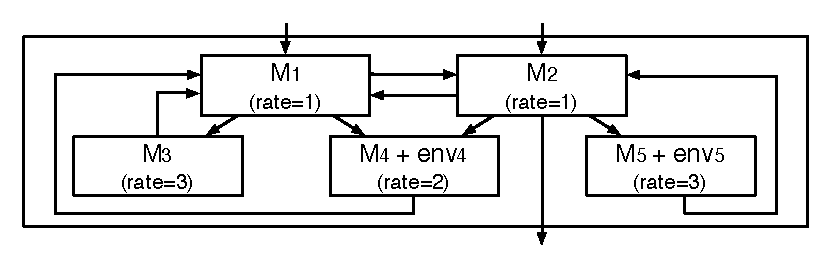
\includegraphics[clip=true,trim=0.3cm 0.4cm 0.3cm 0.4cm,width=1.0\columnwidth]{ensemble.pdf}    
\caption{A multirate machine ensemble $\mathcal{E}$.
%$M_1$ and $M_2$ are slow machines, and 
%%%$M_3$, $M_4$, and $M_5$ are fast machines.
%$\mathit{env}_4$ and $\mathit{env}_5$ are local physical environments 
%of $M_4$ and $M_5$, respectively.
}  \label{fig:ensemble}
\end{figure}



The transitions of all components in an ensemble $\mathcal{E}$
are performed at the same time in lockstep for each iteration.
Each fast machine $M_f$ in $\mathcal{E}$ is \emph{slowed down} 
by performing $k = \mathit{rate}(f)$ internal transitions  in one synchronous step.
A $k$-tuple of outputs from $M_f$  is transformed to 
a single value (e.g., the last value) %or the average of the $k$ values
for a slow machine,
and a single input  from a slow machine
is transformed to a $k$-tuple of inputs for $M_f$
(e.g., a $k$-tuple $(d, d, d, d)$ from a value $d$).
%(e.g., a $k$-tuple $(d, \bot, \ldots, \bot)$ for some ``don't care'' value $\bot$).
%
When a machine has a ``feedback'' wire connected to itself or to another component,
the output becomes an input of the destination component in the \emph{next} iteration.
That is,
the \emph{synchronous composition}  of an ensemble $\mathcal{E}$
is equivalent to a single machine $M_\mathcal{E}$
whose state consists of the states of its subcomponents
and the feedback outputs \cite{mr-pals-journal,pals-tcs}.
For example, 
the synchronous composition $M_\mathcal{E}$ 
of the ensemble $\mathcal{E}$ in Figure~\ref{fig:ensemble} 
is the machine given by the outer box. 
%Notice that $M_\mathcal{E}$ can appear as a component 
%in another multirate ensemble, resulting in hierarchical multirate systems.

%Since a fast machine performs $k$ internal transitions 
%one synchronous step,
%a $k$-tuple of outputs from the fast machine
%must be transformed to a single input (e.g., the last value, or the average of the $k$ values)
%to be read by a slow component.
%Similarly,
%a single output from a slow component must be transformed 
%to a $k$-tuple of inputs for a fast component
%(e.g., 
%a $k$-tuple $(d, \bot, \ldots, \bot)$ for some ``don't care'' value $\bot$).
%An \emph{input adaptor} 
%$\alpha=\{\alpha_j: D'_j \rightarrow D_{i_j}\}_{j\in\{1,\ldots, n\}}$
%for a typed machine $M = (D_i, S, D_o, \delta_M)$
%is a family of functions which determine a desired  value 
%$\alpha_j(d_j) \in D_{i_j}$ for each input 
%port $j$  from an output $d_j \in D_{j}'$
%of another typed machine.


The physical environments of controllers
are specified as periodic dynamic systems \cite{ftscs-journal}.
%
A controller $M$ is a ``periodic'' component 
that collects the state of  its physical environment  $E_M$ using its sensors,
 and has an effect on $E_M$ through its  actuators.
A state of the physical environment $E_M$ 
is given by a tuple $\vec{v} = (v_1,\ldots,v_l) \in \mathbb{R}^l$ 
of its physical parameters $\vec{x} = (x_1, \ldots,x_l)$.
The behavior of $E_M$
is modeled using differential equations that specify \emph{trajectories} 
$\tau_1, \ldots, \tau_l$ of the parameters $\vec{x}$.
A \emph{trajectory} \cite{lynch2003hybrid} of duration $T \in \mathbb{R}_{\geq 0}$ is a function $\tau : [0,T] \rightarrow \mathbb{R}$
that defines the 
continuous behavior of a physical parameter.
%
Let  $\mathcal{T}_T$ denote
the set of all trajectories of 
duration $T$,
and $\vec{\tau}(t) = (\tau_1(t),\ldots,\tau_l(t))$ for a tuple %of trajectories 
$\vec{\tau} = (\tau_1,\ldots,\tau_l) \in \mathcal{T}_T^l$.

A \emph{periodic dynamic system} $E_M = (C, P, T, \Lambda)$ 
specifies all possible trajectories of its parameters $\vec{x}$
during period $T$, % \in \mathbb{R}_{>0}
where:
 \begin{inparaenum}[(i)]
	\item $C$ is a set of \emph{control commands}, representing
          ``actuator outputs'' from %the controller 
          $M$;
	\item $P \subseteq \mathbb{R}^l$ is a set of all possible values 
          of the ``physical 
          parameters'' $\vec{x} = (x_1, \ldots, x_l)$ 
          of  $E_M$; and
	\item $\Lambda \subseteq (C \times P) \times \mathcal{T}_{T}^l$
	is a \emph{physical transition relation} in which
	%that defines possible trajectories of the parameters $\vec{x}$.
	%By definition, 
	$((a, \vec{v}),  \vec{\tau}) \in \Lambda$
	 iff for a control command $a \in C$, % of the controller $M$,
	$E_M$'s physical state gives the trajectory 
	$\vec{\tau} \in \mathcal{T}_{T}^l$ during period $T$
	from a physical state $\vec{v} \in P$
	with $\vec{\tau}(0) = \vec{v}$ at the beginning of a period.
\end{inparaenum}
%
For example,
a physical transition in Figure~\ref{fig:physical-transition} 
defines a trajectory $\tau_i$
from the value $v_i$ to $v_{i+1}$
 according to the control command $a_i$ 
from $M$ during each period.






\begin{figure}
\centering
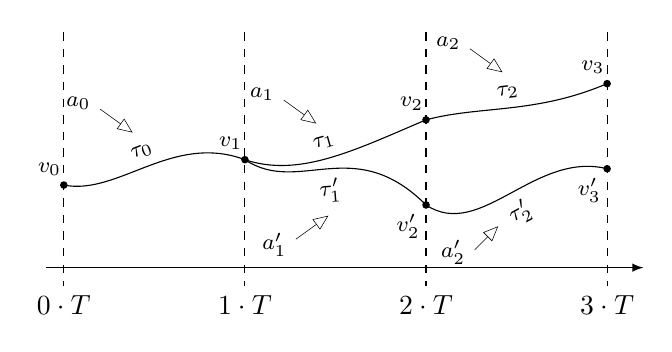
\begin{tikzpicture}[scale=2.3]
%baseline
\draw[-latex,thin] (-0.1,0) -- (3.2,0);
\foreach \x in {0,1,2,3}
\draw[shift={(\x,0)},thin,dashed] (0,1.3) -- (0,-0.1) node[below] { $\x\cdot T$};
%curves
\begin{scope}[yshift=7pt,font=\footnotesize]
\filldraw (0,0.21) circle (0.5pt) node[above,xshift=-1.2ex] {$v_0$};
\draw (0,0.21) .. controls (0.3,0.15) and (0.6,0.5) .. node[above,sloped] (t0) {$\tau_0$} (1,0.35);
\draw[-open triangle 45,very thin] ($(t0.north) + (-0.2,0.15)$) node[left,yshift=2pt] {$a_0$} -- ($(t0.north) + (-0.02,0.02)$);
	\filldraw (1,0.35) circle (0.5pt) node[above,xshift=-1.2ex] {$v_1$};
	\draw (1,0.35) .. controls (1.3,0.25) and (1.6,0.4) .. node[above,sloped] (t1) {$\tau_1$} (2,0.57);
	\draw[-open triangle 45,very thin] ($(t1.north) + (-0.2,0.15)$) node[left,yshift=2pt] {$a_1$} -- ($(t1.north) + (-0.02,0.02)$);
		\filldraw (2,0.57) circle (0.5pt) node[above,xshift=-1.2ex] {$v_2$};
		\draw (2,0.57) .. controls (2.3,0.65) and (2.6,0.6) .. node[above,sloped] (t2) {$\tau_2$} (3,0.77);
		\draw[-open triangle 45,very thin] ($(t2.north) + (-0.2,0.15)$) node[left,yshift=2pt] {$a_2$} -- ($(t2.north) + (-0.02,0.02)$);
			\filldraw (3,0.77) circle (0.5pt) node[above,xshift=-1.2ex] {$v_3$};
	\draw (1,0.35) .. controls (1.3,0.15) and (1.6,0.5) .. node[below,sloped] (t1') {$\tau_1'$} (2,0.1);
	\draw[-open triangle 45,very thin] ($(t1'.south) + (-0.2,-0.15)$) node[left,yshift=-2pt] {$a_1'$} -- ($(t1'.south) + (-0.02,-0.02)$);
		\filldraw (2,0.1) circle (0.5pt) node[below,xshift=-1.5ex] {$v_2'$};
		\draw (2,0.1) .. controls (2.3,-0.1) and (2.6,0.4) .. node[below,sloped] (t2'){$\tau_2'$} (3,0.3);
		\draw[-open triangle 45,very thin] ($(t2'.west) + (-0.15,-0.15)$) node[left,yshift=-1pt] {$a_2'$} -- ($(t2'.west) + (-0.02,-0.02)$);
			\filldraw (3,0.3) circle (0.5pt) node[below,xshift=-1.5ex] {$v_3'$};;;
\end{scope}
\end{tikzpicture}
\caption{A periodic dynamic system $E_M$,
where
$((a_0,v_0), \tau_0) \in \Lambda$, 
$((a_1,v_1), \tau_1) \in \Lambda$, 
$((a_1',v_1), \tau_1') \in \Lambda$, 
%$((a_2,v_2), \tau_2) \in \Lambda$, 
%$((a_2',v_2), \tau_2') \in \Lambda$, 
etc.
}
\label{fig:physical-transition}
\end{figure}





A controller machine $M = (D_i, S, D_o,\delta_{M})$ is considered as 
a \emph{nondeterministic} typed
machine that is
parameterized  by any possible \emph{observable}
behavior of %its physical environment 
$E_M  = (C, P, U, \Lambda)$.
Each state $s \in S$ of $M$ provides
the current control command %of $M$ 
to $E_M$,
denoted by $\pi_C(s) \in C$, and
the ``observed'' physical state by $M$
from a physical state  $\vec{v} \in P$ of $E_M$,
denoted by $\pi_P(s) = \pi_S(\vec{v})$.
%
That is,
the control command $\pi_C(s)$ to $E_M$ is given based on the current state $s$ of $M$,
and
the ``observable'' physical parameters $\pi_S(\vec{v})$ of $E_M$ 
are observed as $\pi_P(s)$ by $M$.
%\footnote{A controller $M$
%is assumed to be tightly integrated with its physical environment $E_M$,
%and thus $M$ can observe or affect $E_M$  immediately;
%for ``remote'' sensors and actuators, % not tightly integrated,
%they  can be considered as parts of another
%controller that communicates with $M$ via a network \cite{ftscs-journal}.}
%
The \emph{environment restriction} %of $M$ by $E_M$ 
is then defined as the machine
$M \restriction E_M = (D_i, S \times P, D_o, \delta_{M \restriction E_M})$,
where 
its transition relation 
$\delta_{M \restriction E_M}$ is constrained by the behavior of $E_M$: i.e.,
%
%a transition 
$((\vec{i}, (s,\vec{v})), ((s',\pvec{v}'), \vec{o}) ) \in \delta_{M \restriction E_M}$ holds
iff:

\begin{itemize}
	\item the $M$'s transition $( (\vec{i}, s), (s', \vec{o}) ) \in \delta_{M}$ holds;
	\item $\pi_P(s) = \pi_S(\vec{v})$ and $\pi_P(s') = \pi_S(\pvec{v}')$ hold; and
	\item the $E_M$'s physical transition 
	$((\pi_C(s), \vec{v}),  \vec{\tau} ) \in \Lambda$
	holds 
	from the current physical state $\vec{v} = \vec{\tau}(0)$ 
	to the next physical state $\pvec{v}' = \vec{\tau}(T)$ during period $T$
	(in other words, the next physical state $\pvec{v}'$ of $E_M$ is 
	reachable from $\vec{v}$  through some trajectory $\vec{\tau}$
	of  $E_M$ based on the current control command $\pi_C(s)$).
\end{itemize}










%%%
\subsection{Delta-Complete SMT}

\textbf{Sean, please write a brief overview of dReal}
\newpage


%%%%
%%%%
\section{CPS for Turning an Airplane}

This section illustrates a distributed hybrid system
for turning an airplane to an angle specified by a pilot,
through a distributed control system to move the ailerons and the rudder 
of the airplane
in a synchronous way.
An aileron is a movable surface attached to  each wing, and a rudder is a movable surface attached to the vertical tail.
%
The controllers 
for the ailerons and the rudder operate at different rates,
and the main controller orchestrates the sub-controllers 
to achieve a smooth turn
according to a specified goal angle.
%
The continuous dynamics of the turning control system
is governed by \emph{nonlinear} differential equations
that involve the angles of the ailerons and the rudder.




An airplane typically makes a turn by operating its two ailerons in opposite directions.
The difference between the lift forces in the left and the right wings
then makes the airplane roll toward a desired direction, 
so that the airplane moves in a circular motion 
because of  the centripetal lift force 
generated by the two wings.
However, the rolling of the airplane also causes
\emph{adverse yaw}, making the airplane sideslip in the opposite direction of a roll.
This undesirable side effect can be countered by 
generating the opposing side lift force on the vertical tail
by moving the rudder of the airplane.
To make a \emph{coordinated turn} effectively, the yaw angle $\beta$ should
always stay at $0^\circ$
during a turn.




Under some simplifying assumptions,%
\footnote{E.g., the wings of the airplane have no dihedral angle, 
the speed $v$ of the airplane is constant, 
the altitude does not change, there is no turbulence, etc.}
the direction angle $\psi$, the roll angle $\phi$, and the yaw angle $\beta$
can be modeled by the following nonlinear differential equations 
including 
the angle $x_l$ of the left aileron,
the angle $x_r$ of the right aileron, and 
the angle $x_v$ of the rudder
\cite{ftscs-journal}:
%
\begin{align}
\frac{\mathrm{d}\psi}{\mathrm{d}t} &= (g / v) \cdot \tan \phi
\label{eq:dir}
\\
(\frac{\mathrm{d}\phi}{\mathrm{d}t})^2 &=
\frac{C_{l,w} (x_r - x_l)}{W \cdot L_\mathit{Wing}}
\label{eq:roll}
\\
(\frac{\mathrm{d}\beta}{\mathrm{d}t})^2 &=
\frac{C_d \cdot C_{l,w}  ( x_r -  x_l)}{W \cdot L_\mathit{Wing}}
 + \frac{C_{l,v} \cdot x_v}{W \cdot L_\mathit{Airplane}}
 \label{eq:yaw}
\end{align}
%
where $(\frac{\mathrm{d}\phi}{\mathrm{d}t})^2 = f(t)$
means that 
$\frac{\mathrm{d}\phi}{\mathrm{d}t} = \sqrt{f(t)}$ if $f(t) \geq 0$,
and
$\frac{\mathrm{d}\phi}{\mathrm{d}t} = - \sqrt{- f(t)}$ if $f(t) < 0$.
In the equation, $g$ is the gravity constant, $v$ is the speed of the airplane,
$W$ is the mass of the airplane, 
 $L_\mathit{Wing}$ is the length of the left or the right wing,
 $L_\mathit{Airplane}$ is the length of the airplane,
 $C_{l,w}$ is the lift constant for the horizontal wings,
 $C_{l,v}$ is the lift constant for the vertical tail wing,
 and  $C_d$ is the drag ratio.%
 \footnote{The values of the constants  $C_{l,w}$,  $C_{l,v}$, and $C_d$
 depend on the shape of the wing or the aircraft.}

 




Using the Multirate PALS methodology,
we only specify  a synchronous model,
namely,  a multirate ensemble $\mathcal{E}$ that consists of 
the main controller and the three sub-controllers.
These controllers in $\mathcal{E}$ defines 
the system's \emph{discrete} behavior,
while their local physical environments
%given by periodic dynamic systems,
defines the system's continuous behavior.
%
Multirate PALS then generates
the \emph{correct-by-construction}   
implementation  
$\mathcal{A}(\mathcal{E}, T, \Gamma)$,
given a global period $T$ and performance bounds 
$\Gamma$ on the network infrastructure.
%
The synchronous model $\mathcal{E}$ %in this section
is adapted from \cite{ftscs-journal} 
for precisely specifying \emph{immediate correlation}
between the physical environments of the controllers.
%
The architecture of the system is illustrated in Figure~\ref{fig:airplane-ctrl}.

\begin{figure}
\centering
\tikzstyle{comp}=[draw,thick,rounded corners=4pt,text centered,execute at begin node=\small]
\tikzstyle{env}=[draw,dashed,rounded corners=4pt,text centered,execute at begin node=\small]
\tikzstyle{conn}=[thick,-latex,font=\scriptsize]
\tikzstyle{envconn}=[very thin,-open triangle 45,font=\scriptsize]
\begin{tikzpicture}[scale=0.9,every node/.style={transform shape}] 
%components
\node (main) [comp,text width=10ex,minimum height=36ex] 
	{{Main\\ controller} ($60\, \mathrm{ms}$, $\mathit{rate}$ = $1$)}; 
\path (main.east |- main.north) + (17ex,-5.5ex) node (left) [comp,text width=13ex,minimum height=11ex] 
	{{Left aileron\\ subcontroller}\\ ($15\, \mathrm{ms}$, $\mathit{rate}$ = $4$)}; 
\path (main.east) + (17ex,0) node (vert) [comp,text width=13ex,minimum height=11ex] 
	{{Rudder\\ subcontroller}\\ ($20\, \mathrm{ms}$, $\mathit{rate}$ = $3$)}; 
\path (main.east |- main.south) + (17ex,5.5ex) node (right) [comp,text width=13ex,minimum height=11ex] 
	{{Right aileron\\ subcontroller}\\ ($15\, \mathrm{ms}$, $\mathit{rate}$ = $4$)}; 
%comp connections
\draw [conn,latex-] (main.west |- main.north) + (3ex,0)-- node{ }+(3ex,3ex) node[above] {$\mathit{goal}_\psi$};
\draw [conn] (main.east |- main.north) + (-3ex,0)-- node{ }+(-3ex,3ex) node[above] {$\psi$};
\draw[conn] ($(main.east |- left)+(0,1ex)$) -- node[above] {$\mathit{goal}_l$} ($(left.west |- left)+(0,1ex)$);
\draw[conn] ($(left.west |- left)+(0,-1ex)$) -- node[below] {$a_l$} ($(main.east |- left)+(0,-1ex)$);
\draw[conn] ($(main.east |- vert)+(0,1ex)$) -- node[above] {$\mathit{goal}_v$} ($(left.west |- vert)+(0,1ex)$);
\draw[conn] ($(left.west |- vert)+(0,-1ex)$) -- node[below] {$a_v$} ($(main.east |- vert)+(0,-1ex)$);
\draw[conn] ($(main.east |- right)+(0,1ex)$) -- node[above] {$\mathit{goal}_r$} ($(left.west |- right)+(0,1ex)$);
\draw[conn] ($(left.west |- right)+(0,-1ex)$) -- node[below] {$a_r$} ($(main.east |- right)+(0,-1ex)$);
%physical envs
\path (main.west) + (-9.5ex,0ex) node (main-env) [env,text width=6ex,minimum height=36ex] 
	{$E_\mathit{main}$}; 
\path (left.east) + (14ex,0ex) node (left-env) [env,text width=8ex,minimum height=11ex] 
	{$E_\mathit{left}$}; 
\path (vert.east) + (14ex,0ex) node (vert-env) [env,text width=8ex,minimum height=11ex] 
	{$E_\mathit{rudder}$}; 
\path (right.east) + (14ex,0ex) node (right-env) [env,text width=8ex,minimum height=11ex] 
	{$E_\mathit{right}$}; 
%physical env conns
\draw[envconn] ($(main-env.east |- main-env.north)+(0,-8ex)$)
	-- node[above] {$\psi$} ($(main.west |- main-env.north)+(0,-8ex)$);
\draw[envconn] (main-env.east)
	-- node[above] {$\phi$} (main.west);
\draw[envconn] ($(main-env.east |- main-env.south)+(0,8ex)$)
	-- node[above] {$\beta$} ($(main.west |- main-env.south)+(0,8ex)$);
\draw[envconn] ($(left.east |- left-env)+(0,1ex)$) 
	-- node[above] {$\mathit{rate}_l$} ($(left-env.west |- left-env)+(0,1ex)$);
\draw[envconn] ($(left-env.west |- left-env)+(0,-1ex)$) 
	-- node[below] {$x_l$} ($(left.east |- left-env)+(0,-1ex)$);
\draw[envconn] ($(vert.east |- vert-env)+(0,1ex)$) 
	-- node[above] {$\mathit{rate}_v$} ($(vert-env.west |- vert-env)+(0,1ex)$);
\draw[envconn] ($(vert-env.west |- vert-env)+(0,-1ex)$) 
	-- node[below] {$x_v$} ($(vert.east |- vert-env)+(0,-1ex)$);
\draw[envconn] ($(right.east |- right-env)+(0,1ex)$) 
	-- node[above] {$\mathit{rate}_r$} ($(right-env.west |- right-env)+(0,1ex)$);
\draw[envconn] ($(right-env.west |- right-env)+(0,-1ex)$) 
	-- node[below] {$x_r$} ($(right.east |- right-env)+(0,-1ex)$);
\end{tikzpicture}
\caption{The airplane turning control system.} \label{fig:airplane-ctrl}
\end{figure}

\subsection{The Aileron and Rudder Controllers}

A sub-controller receives a desired angle of the wing
from the main controller,
and gradually moves the surface of the wing toward the goal angle.
The continuous movement of the angle is modeled by its physical environment.
E.g., 
the left aileron sub-controller receives the goal angle $\mathit{goal}_l$ from the main controller, 
and sets the moving rate $\mathit{rate}_l$
  for the physical environment $E_\mathit{left}$
(that is less than or equal to the maximal rate $\mathit{max}_l$).
%
Meanwhile, the wing angle $x_l$ in $E_\mathit{left}$  changes according to the differential equation
$\frac{\mathrm{d} x_l}{\mathrm{d}t} = \mathit{rate}_l$ during a $15\,\mathrm{ms}$ period.
%
The other sub-controllers are similar,
except their periods and the maximal rates.

The left aileron sub-controller  can be specified 
as the typed machine 
$M_\mathit{left} = (\mathbb{R}, \mathbb{R}^2, \mathbb{R}, \delta_{\mathit{left}})$.
The machine $M_\mathit{left}$ has one input port to receive $\mathit{goal}_l \in \mathbb{R}$,
and one output port to report the observed angle. % of the wing.
A state $(\mathit{rate}_l, a_l) \in \mathbb{R}^2$ is a pair of the current rate $\mathit{rate}_l$ and the observed angle $a_l$.
A transition $((\mathit{goal}_l, (r, a)), ((r', a'),a)) \in  \delta_{\mathit{left}}$
holds iff 
\[
r' = \sign(\mathit{goal}_l - a) \cdot \min(\abs(\mathit{goal}_l - a) / 15, \mathit{max}_l)
\]
where $\sign(v) = \ite{v \neq 0}{v / abs(v)}{0}$, and
$a' \in \mathbb{R}$ is the \emph{next}  observed angle after $15\,\mathrm{ms}$ elapsed,
determined by the physical environment $E_\mathit{left}$.

The periodic dynamic system 
$E_\mathit{left} = (\mathbb{R}, \mathbb{R}, 15\,\mathrm{ms}, \Lambda_\mathit{left})$
has the control command set $\mathbb{R}$ for the moving rate $\mathit{rate}_l$,
and the state set $\mathbb{R}$ for the surface angle of the left aileron.
The physical transition 
$( (\mathit{rate}_l, a_l), x_l ) \in \Lambda_{E_\mathit{left}}$ holds
iff there exists a trajectory $x_l \in \mathcal{T}_{15}$ such that
$\frac{\mathrm{d} x_l}{\mathrm{d}t} = \mathit{rate}_l$ and $x_l(0) = a_l$
(i.e., the wing angle  $x_l$ varies 
according to the differential 
equation $\frac{\mathrm{d} x_l}{\mathrm{d}t} = \mathit{rate}_l$
from the current angle $x_l(0) = a_l$
during a $15\,\mathrm{ms}$ period).

The combined behavior is then given by the environment restriction machine
$M_\mathit{left} \restriction E_\mathit{left} = (\mathbb{R}, \mathbb{R}^2 \times \mathbb{R}, \mathbb{R}, \delta_{M_\mathit{left} \restriction E_\mathit{left}})$.
A transition 
$((\mathit{goal}_l, (r, a, a))), ((r',a', a'), a) ) 
\in \delta_{M_\mathit{left} \restriction E_\mathit{left}}$ 
holds iff
the transition $( (\mathit{goal}_l, (r,a)), ((r',a'),a) ) \in \delta_{\mathit{left}}$
of $M_\mathit{left}$
and the physical transition 
$((r, a), x_l) \in \Lambda_{\mathit{left}}$ of $E_\mathit{left}$ hold
with the current surface angle $x_l(0) = a$ and the next angle $x_l(15) = a'$,
where the control commands to $E_\mathit{left}$ are defined by the projection function $\pi_C(r,a) = r$,
and the observed parameters of $E_\mathit{left}$ by $M_\mathit{left}$
are defined using the projection functions $\pi_P(r,a) = a$ and $\pi_S(a) = a$.
%
Notice that $M_\mathit{left}$ is nondeterministic
since the next observed angle $a'$ is not specified,
whereas
$M_\mathit{left} \restriction E_\mathit{left}$ is deterministic.




\subsection{The Main Controller}

The main controller $M_\mathit{main}$ receives 
a desired direction of the airplane (specified by the pilot),
and determines the new surface angles of the sub-controllers
for a coordinated turn. 
%
The direction angle $\psi$, the roll angle $\phi$, and the yaw angle $\beta$,
governed by the nonlinear differential equations (\ref{eq:dir})--(\ref{eq:yaw}),
consist in the physical environment $E_\mathit{main}$.
For each step, the main controller receives the goal direction
$\mathit{goal}_\psi$ from the pilot 
and the observed surface angles $(a_l, a_v, a_r)$
from the aileron and the rudder sub-controllers,
and then sends the new goal angles 
$(\mathit{goal}_l, \mathit{goal}_v, \mathit{goal}_r)$ to the sub-controllers,
based on the current observed position angles $(\psi, \phi, \beta)$.


The position angles $\psi$, $\phi$, and $\beta$ correlate
physically with the surface angles $x_l$, $x_r$, and $x_v$,
because the differential equations (\ref{eq:dir})--(\ref{eq:yaw}) contain 
the variables $x_l$, $x_r$, and $x_v$.
These angles are \emph{not} constants,
since the sub-controllers gradually  moves the surfaces of the wings.
Therefore, the physical environment $E_\mathit{main}$
also includes the parameters $x_l$, $x_r$, and $x_v$
for its physical states.
It is worth noting that the surface angles $x_l$, $x_r$, and $x_v$
\emph{cannot} be directly observed by the main controller, 
because the sub-controllers are distributed;
however, the main controller can still use the surface angles $(a_l, a_v, a_r)$,
observed by the sub-controllers and received in the input ports of the main controller.
 
The physical environment of $M_\mathit{main}$
is specified by the periodic dynamic system
$E_\mathit{main} = (\{\ast\}, \mathbb{R}^6, 60\,\mathrm{ms}, \Lambda_{\mathit{main}})$.
The singleton set $\{\ast\}$ indicates 
that $M_\mathit{main}$ gives \emph{no} control commands to $E_\mathit{main}$.
A physical state of $E_\mathit{main}$
is a $6$-tuple in $\mathbb{R}^6$ 
to denote $(\psi,  \phi, \beta, x_l, x_v, x_r)$.
A physical transition
$((\ast, (d,  l, y, a_l, a_v, a_r)), (\psi,  \phi, \beta, x_l, x_v, x_r)) \in \Lambda_{\mathit{main}}$
holds
iff there are trajectories $\psi,  \phi, \beta, x_l, x_v, x_r \in \mathcal{T}_{60}$
of duration $60\,\mathrm{ms}$,
satisfying 
$(\psi,  \phi, \beta, x_l, x_v, x_r)(0) = (d,  l, y, a_l, a_v, a_r)$
and
the aeronautics 
differential equations~(\ref{eq:dir})--(\ref{eq:yaw}). 
Note that 
the trajectories $x_l$, $x_v$, and $x_r$ of the three surface angles 
are determined by the subcontrollers.

We consider a control logic to decide 
the new angles of the ailerons and the rudder
%only based on the observed position angles and the goal direction
by control functions \cite{ftscs-journal}.
%
The function $f_\phi(l, d, \mathit{goal}_\psi)$
computes the desired roll angle $\phi$,
 based on 
the observed roll angle $l$, the observed direction $d$, and 
the goal direction $\mathit{goal}_\psi$.
%
The function
 $f_{R}(l, \mathit{goal}_\phi)$
computes the desired angle of the right aileron,
based on the observed roll angle $l$ and the goal roll angle $\mathit{goal}_\phi$
(the left aileron angle is %always 
exactly opposite to the right aileron angle).
%
The function $f_V(y)$ returns the desired rudder angle,
based on the observed yaw angle $y$. % (the goal yaw angle is $0^\circ$).
For example,
in \cite{ftscs-journal}:
\[
\begin{medsize}
\begin{aligned}
f_\phi(l, d, \mathit{g}_\psi) &= 
\mathrm{ite}(\abs(h - l) > 1.5, l +  1.5 \cdot\sign(h-l), h)
\\
f_{R}(l, \mathit{g}_\phi) &=
\sign(q)\cdot \mathrm{ite}(\abs(q) > 1, \min(0.3 \cdot \abs(q), 45), 0.3 \, q^2)
\\
f_V(y) &=
\begin{aligned}[t]
\sign(-y)\cdot \mathrm{ite}(\abs(y) > 1, \min(0.8 \cdot \abs(y), 30), 0.8 \, y^2),
\end{aligned}
\end{aligned}
\end{medsize}
\]
where $h = 0.32 \cdot (\mathit{g}_\psi - d)$,
$q = \mathit{g}_\phi - l$,
and $\mathrm{ite}(\mathit{cond},e_1,e_2)$ is the conditional function.


The main controller is then specified 
as the typed machine $M_\mathit{main} = (\mathbb{R}^4, \mathbb{R}^3, \mathbb{R}^4, \delta_\mathit{main})$,
where
its state has observed %position
 angles $(d, l, y) \in \mathbb{R}^3$,
and a transition
$(((\mathit{goal}_\psi, a_l, a_v, a_r), \allowbreak (d,l,y)), \allowbreak
((d', l', y'), \allowbreak (d, \mathit{goal}_l, \mathit{goal}_v, \mathit{goal}_r))) \in \delta_\mathit{main}$
holds iff 
$\mathit{goal}_r = f_{R}(l, f_\phi(l, d, \mathit{goal}_\psi))$,
$\mathit{goal}_l = - \mathit{goal}_r$,  
$\mathit{goal}_v = f_V(y)$,
and
%provided that 
$(d', l', y')$ are the next observed position angles 
after $60\,\mathrm{ms}$ elapsed,
determined by $E_\mathit{main}$.
Then, the environment restriction $M_\mathit{main} \restriction E_\mathit{main}$
 defines the combined behavior in an expected way,
where there are no control commands (i.e., $\pi_C(d,l,y) = \ast$)
and
the observed parameters 
are given by
$\pi_P(d,l,y) = (d,l,y)$ and $\pi_S(d,  l, y, a_l, a_v, a_r) = (d,l,y)$.





 


%%%%
%%%%
\section{SMT-based Analysis}

This section explains how the distributed airplane turning  
controller
can be analyzed by using SMT  techniques.
We first \emph{symbolically} represent 
the behavior  of the synchronous model $\mathcal{E}$
and  its physical environments as logic formulas up to a given time bound. 
The safety of the system can then be verified 
 by checking the satisfiability of these formulas using a SMT solver, 
 provided that the safety requirements are also expressed as logic formulas.
 %
The generated formulas include 
may instances of the nonlinear differential equations (\ref{eq:dir})--(\ref{eq:yaw}).
Thanks to $\delta$-complete SMT solving, 
the satisfiability of such formulas can be decided 
up to a given error bound $\delta > 0$.
Unlike the previous work \cite{ftscs-journal}
that numerically simulates the behavior of $\mathcal{E}$, 
using this method we can verify the system 
with respect to 
an infinite number of  system parameters (e.g., speed, weight, etc)
and arbitrary pilot behaviors.

%This also involves a nontrivial extension of  \texttt{dReal},
%since, due to the distributed nature of the system,
%the generated formula may include uninterpreted real function symbols
%that are not supported by the existing \texttt{dReal} interface.

The major challenge is to deal with physical correlations
between the physical environments of the main controller and the sub-controllers.
The continuous dynamics of the position angles $(\psi, \phi, \beta)$
also depends on the surface angles $(x_l, x_v, x_r)$ of the ailerons and the rudder. 
Since our model is a multirate system,
the moving rate of the surface angles can be changed by the sub-controllers
\emph{at different moments}
(e.g., a $15\,\mathrm{ms}$ period for the ailerons, and a $20\,\mathrm{ms}$ period for the rudder).
This makes it difficult to generate a formula of the main controller (having a $60\,\mathrm{ms}$ period) in a modular way,
since they must take into account those different flows of $(x_l, x_v, x_r)$.
Hence, we have extended the \texttt{dReal} SMT solver
to directly handle such \emph{parameterized} differential equations over different flows
in input formulas.



 


%%%
\subsection{Generating Formulas}

For a machine  $M = (D_i,S,D_o,\delta_M)$
with $n$ input ports and $m$ output ports,
its transition $\delta_M \subseteq (D_i \times S) \times (S \times D_o)$
can be expressed as a first order logic formula of the form
$\varphi_{M}(y_{i_1},\ldots,y_{i_n}\shortmid
y_{s_1},\ldots,y_{s_k}\shortmid
y_{s_1}',\ldots,y_{s_k}'\shortmid
y_{o_1},\ldots,y_{o_m}),
$ with
the variables $y_{i_1},\ldots,y_{i_n}$ for the inputs,
the variables $y_{s_1},\ldots,y_{s_k}$  for the current discrete state, 
$y_{s_1}',\ldots,y_{s_k}'$  for the next discrete state, and 
$y_{o_1},\ldots,y_{o_m}$  for the outputs.
That is,
$\varphi_{M}(\vec{i}\shortmid s\shortmid s'\shortmid  \vec{o})$
iff $( (\vec{i}, s), (s', \vec{o}) ) \in \delta_{M}$.

For the sake of simplicity, 
we annotate each variable with 
a machine identifier and a model time $t$. %when the transition happens.
For example, the formula $\varphi_{M_\mathit{left}}$
for the left aileron controller (at time $t$) is:
\[
\begin{medsize}
\begin{aligned}
&
\varphi_{M_\mathit{left}}(y_{g}^{l;t} \shortmid  y_{r}^{l;t}, y_{a}^{l;t} 
	\shortmid y_{r}^{l;t + 15}, y_{a}^{l;t + 15} \shortmid y_{o}^{l;t})
\\
\equiv\quad
&
y_{o}^{l;t} = y_{a}^{l;t} \;\wedge
\\
&
y_{r}^{l;t + 15} = \sign(y_{g}^{l;t} - y_{a,L}^{t}) \cdot \min(\abs(y_{g}^{l;t} - y_{a,L}^{t}) / 15, \mathit{max}_l)
\end{aligned}
\end{medsize}
\]
and $\varphi_{M_\mathit{main}}$ for the main controller (at time $t$) is:
\[
\begin{medsize}
\begin{aligned}
&
\begin{aligned}
\varphi_{M_\mathit{main}}(
	&y_{\mathit{g}_\psi}^{m;t}, y_{a_l}^{m;t}, y_{a_v}^{m;t}, y_{a_r}^{m;t}  \shortmid
	y_d^{m;t}, y_l^{m;t}, y_y^{m;t} \shortmid
\\
	&y_d^{m;t+60}, y_l^{m;t+60}, y_y^{m;t+60} \shortmid
	y_o^{m;t}, y_{g_l}^{m;t}, y_{g_v}^{m;t}, y_{g_r}^{m;t})
\end{aligned}
\\
\equiv\quad
&
y_o^{m;t} = y_d^{m;t} 
\;\;\wedge\;\;
y_{g_l}^{m;t} = - y_{g_r}^{m;t}
\;\;\wedge\;\;
y_{g_v}^{m;t} = f_V(y_y^{m;t})
\;\;\wedge\;\;
\\
&
y_{g_r}^{m;t} = f_{R}(y_l^{m;t}, f_\phi(y_l^{m;t}, y_d^{m;t}, y_{\mathit{g}_\psi}^{m;t}))
\end{aligned}
\end{medsize}
\]






The physical transition relation $\Lambda$ 
of a periodic dynamic system
$E_M = (C, P, T, \Lambda)$
can be expressed as a formula
of the form
$\varphi_{E_M}(
y_{C_1},\ldots,y_{C_j}\shortmid
y_{v_1}, \ldots, y_{v_l}\shortmid
y_{v_1}', \ldots, y_{v_l}')
$
with
the variables $y_{C_1},\ldots,y_{C_j}$  for control commands,
the variables  $y_{v_1}, \ldots, y_{v_l}$  for the current values of the physical parameters,
and 
$y_{v_1}', \ldots, y_{v_l}'$ for the next parameter values after time $T$ elapsed.
That is,
$\varphi_{E_M}(a\shortmid \vec{v}\shortmid \vec{v}')$
iff
$\vec{v} = \vec{\tau}(0)$, 
$\vec{v}' = \vec{\tau}(T)$, and 
$((a, \vec{v}),  \vec{\tau}) \in \Lambda$ hold.

For differential equations,
their solution functions can be written in the formula 
using integral operators and syntactic flow assignments.
A solution function can be parameterized by
\emph{time-bounded flow parameters}.
%
For example, the formula for the main controller's physical environment
 (at time $t$): 
% $\varphi_{E_{M_\mathit{main}}}$:
\[
\begin{medsize}
\begin{aligned}
	\begin{multlined}
	\varphi_{E_{M_\mathit{main}}}(\ast  \shortmid
		 y_d^{E_m;t},  y_l^{E_m;t}, y_y^{E_m;t}, y_{a_l}^{E_m;t}, y_{a_v}^{E_m;t}, y_{a_r}^{E_m;t}  \shortmid  \\
		 y_d^{E_m;t+60},  y_l^{E_m;t+60}, y_y^{E_m;t+60}, y_{a_l}^{E_m;t+60}, y_{a_v}^{E_m;t+60}, y_{a_r}^{E_m;t+60} )
	\end{multlined}
\end{aligned}
\end{medsize}
\]
is expressed
using the aeronautics equations~(\ref{eq:dir})--(\ref{eq:yaw})
and the flow parameters $\mathit{fp}_{x_l}$,
$\mathit{fp}_{x_v}$, and $\mathit{fp}_{x_r}$
bounded in the time interval $[t, t+60]$ as follows:
\[
\left[
\begin{medsize}
\begin{aligned}
y_d^{E_m;t+60}\\ 
y_l^{E_m;t+60}\\
y_y^{E_m;t+60}\\
y_{a_l}^{E_m;t+60}\\
y_{a_v}^{E_m;t+60}\\
y_{a_r}^{E_m;t+60}
\end{aligned}
\end{medsize}
\right]
=
\left[
\begin{medsize}
\begin{aligned}
y_d^{E_m;t}\\ 
y_l^{E_m;t}\\
y_y^{E_m;t}\\
y_{a_l}^{E_m;t}\\
y_{a_v}^{E_m;t}\\
y_{a_r}^{E_m;t}
\end{aligned}
\end{medsize}
\right]
+
\bigintssss_{0}^{60}
\left[
\begin{medsize}
\begin{aligned}
\mathrm{Equation~(\ref{eq:dir})}
\\
\mathrm{Equation~(\ref{eq:roll})}
\\
\mathrm{Equation~(\ref{eq:yaw})}
 \\
\mathit{fp}_{x_l}{[t,t+60]}
\\
\mathit{fp}_{x_v}{[t,t+60]}
\\
\mathit{fp}_{x_r}{[t,t+60]}
\end{aligned}
\end{medsize}
\right]
\mathrm{d}t
\]
The formulas for the sub-controllers' physical environments
syntactically assign the relevant flows  to the parameters;
e.g., for the left aileron controller, four consecutive instances of the following formula 
for $u \in \{t, t + 15, t + 30, t + 45\}$:
\[
\begin{medsize}
\begin{aligned}
&
\varphi_{E_{M_\mathit{left}}}(y_{r}^{E_l;u} \shortmid y_{a}^{E_l;u} \shortmid y_{a}^{E_l;u + 15})
\\ 
\equiv\quad&
y_{a}^{E_l;u + 15} = y_{a}^{E_l;u} + \int_{0}^{15} y_{r}^{E_l;u} \mathrm{d}t
\;\wedge\;
\mathit{fp}_{x_l}{[t,t+15]} = [y_{r}^{E_l;u}]
\end{aligned}
\end{medsize}
\]
Theoretically, 
the formula is in many-sorted first order logic
where flows are first order terms of a distinguished sort
and the integral operator takes such flows as its arguments.


The correspondence between a controller and its physical environments,
and the connections between input ports and output ports 
can be encoded
by adding   
%appropriate 
\emph{equality conditions} between the corresponding variables
in the formula.
For example, 
given a state $(r, a)$ of the left 
aileron controller $M_\mathit{left}$,
the control command to $E_\mathit{left}$ is $\pi_C(r,a) = r$,
and the observed parameter is $\pi_P(r,a) = a$.
Therefore, we add the 
equality conditions 
$y_{r}^{l;t} = y_{r}^{E_l;t}$ and $y_{a}^{l;t} = y_{a}^{E_l;t}$.
Likewise, we add $(y_d^{m;t}, y_l^{m;t}, y_y^{m;t}) = (y_d^{E_m;t},  y_l^{E_m;t}, y_y^{E_m;t})$
for the main controller $M_\mathit{main}$.
An output $\mathit{goal}_l$ of $M_\mathit{main}$
becomes the input of $M_\mathit{left}$ in the \emph{next} synchronous step.
Since the period of $M_\mathit{main}$ is four times longer than the period of $M_\mathit{left}$,
we add 
the conditions 
$y_{g_l}^{m;t} = y_{g}^{l;t + 60} =  y_{g}^{l;t + 75} 
=  y_{g}^{l;t + 90} = y_{g}^{l;t + 105}$.
%On the other hand,
An output $a$ of  $M_\mathit{left}$
becomes the input of $M_\mathit{main}$ in the next step,
and because $M_\mathit{main}$ takes the last value of a $k$-vector of inputs,
we add the condition  $y_{a_l}^{m;t + 60} = y_{g}^{l;t + 45}$.




To perform bounded model checking of the synchronous model $\mathcal{E}$,
we generate the logic formulas for the controllers and their physical environments
up to a given time bound $T \in \{60 n \mid n \in \mathbb{N}\}$,
and then add the corresponding equality conditions.
The safety property %of $\mathcal{E}$ 
is that 
the yaw angle $\beta$ is always close to $0^\circ$.
Using the variable $y_y^{m;t}$ to denote the observable yaw angle at time $t$,
this property can be express as the conjunction of each formula $y_y^{m;t} < \epsilon$ for 
a certain $\epsilon > 0$ and $t \in \{60 n < T\mid n \in \mathbb{N}\}$.
The system $\mathcal{E}$ can violate the safety property 
at time $T$
iff the generated formula and $y_y^{m;T} \geq \epsilon$
is satisfiable at the same time,
which is automatically checkable using the \texttt{dReal} solver.
We repeat this process by iteratively incrementing the time bound $T$.
This process is \emph{refutationally complete},
in the sense that 
if the system $\mathcal{E}$ violates the safety property,
then  the process can detect the violation and generate a counterexample.











%%%
\subsection{Checking Satisfiability}

\textbf{Sean, please briefly write something about the new implementation}
\newpage



%%%%
%%%%
\section{Evaluations}

%%%
\subsection{Symbolic Analysis}

%%%
\subsection{Concrete Analysis}

%%%
\subsection{Limitations}

liveness properties

continuous invariants $\forall \beta(t) < \epsilon$

more general physical correlations





%%%%
%%%%
%\section{Concluding Remarks}


%%%%
\bibliographystyle{abbrv}
\bibliography{kbae-bib,../ref}

\end{document}
